\graphicspath{{chapters/ch-gsn/figures/}}

\chapter{GSN an Evaluation}%: Stream Processing Infrastructure for Large-scale Interconnected Streaming World



\section{Evaluation \footnote{The evaluation results in this section correspond to GSN release 0.90}}
\label{sec:evaluation}

GSN aims at providing a zero-programming and efficient infrastructure for
large-scale interconnected sensor networks. To justify this claim we
experimentally evaluate the throughput of the local sensor data processing and
the performance and scalability of query processing as the key influencing
factors.  As virtual sensors are addressed explicitly and GSN nodes communicate
directly in a point-to-point (peer-to-peer) style, we can reasonably
extrapolate the experimental results presented in this section to larger
network sizes.  For our experiments, we used the setup shown in
Figure~\ref{fig:ExperimentalSetup}.

The GSN network consisted of 5 standard Dell desktop PCs with Pentium 4, 3.2GHz
Intel processors with 1MB cache, 1GB memory, 100Mbit Ethernet, running Debian
3.1 Linux with an unmodified kernel 2.4.27. For the storage layer use standard
MySQL 5.18.  The PCs were attached to the following sensor networks as shown in
Figure~\ref{fig:ExperimentalSetup}.

\begin{itemize}
  
\item A sensor network consisting of 10 Mica2 motes, each mote being equipped
  with light and temperature sensors. The packet size was configured to 15
  Bytes (data portion excluding the headers).
  
\item A sensor network consisting of 8 Mica2 motes, each equipped with light,
  temperature, acceleration, and sound sensors. The packet size was
  configured to 100 Bytes (data portion excluding the headers).  The maximum
  possible packet size for TinyOS 1.x packets of the current TinyOS
  implementation is 128 bytes (including headers).
  
\item A sensor network consisting of 4 Tiny-Nodes (TinyOS compatible motes
  produced by Shockfish, \url{http://www.shockfish.com/}), each equipped with a
  light and two temperature sensors with TinyOS standard packet size of 29
  Bytes.
  
\item 15 Wireless network cameras (AXIS 206W) which can capture 640x480 JPEG
  pictures with a rate of 30 frames per second. 5 cameras use the highest
  available compression (16kB average image size), 5 use medium compression
  (32kB average image size), and 5 use no compression (75kB average image
  size). The cameras are connected to a Linksys WRT54G wireless access point
  via 802.11b and the access point is connected via 100Mbit Ethernet to a GSN
  node.
  
\item A Texas Instruments Series 6000 S6700 multi-protocol RFID reader with
  three different kind of tags, which can keep up to 8KB of data.
  128 Bytes capacity.
  
\end{itemize}

The motes in each sensor network form a sensor network and routing among the
motes is done with the surge multi-hop ad-hoc routing algorithm provided by
TinyOS.

\begin{figure}%[htb]
  \centering
  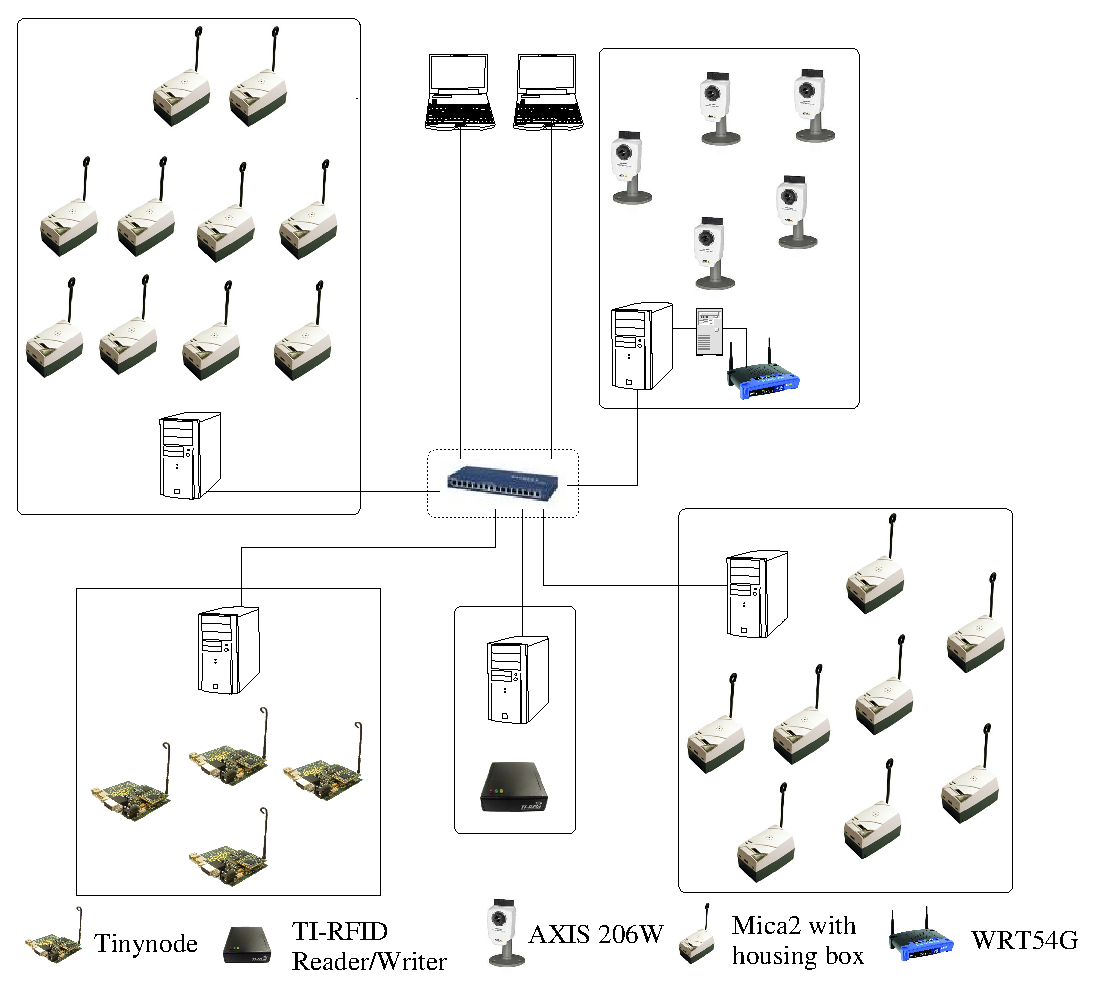
\includegraphics[width=0.8\columnwidth]{setup}
  \caption{Experimental setup}
  \label{fig:ExperimentalSetup}
\end{figure}


\subsection{Internal processing time}
\label{sec:exepr-eval}

In the first experiment we wanted to determine the internal processing time a
GSN node requires for processing sensor readings, i.e., the time interval when
the wrapper gets the sensor data until the data can be provided to clients by
the associated virtual sensor. This delay depends on the size of the sensor
data and the rate at which the data is produced, but is independent of the
number of clients wanting to receive the sensor data. Thus it is a lower bound
and characterizes the efficiency of the implementation. 

We configured the 22 motes and 15 cameras to produce data every 10, 25, 50,
100, 250, 500, and 1000 milliseconds. As the cameras have a maximum rate of 30
frames/second, i.e., a frame every 33 milliseconds, we added a proxy between
the GSN node and the WRT54G access point which repeated the last available
frame in order to reach a frame interval of 10 milliseconds. All GSN instances
used the Sun Java Virtual Machine (1.5.0 update 6) with memory restricted to
64MB.

The experiment was conducted as follows: All motes and cameras were set to the
same rate and produced data for 8 hours and we measured the processing delay.
This was repeated 3 times for each rate and the measurements were averaged.
Figure~\ref{fig:TimeTriggeredLoad} shows the results of the experiment for the
different data sizes produced by the motes and the cameras.

\begin{figure}%[htb]
  \centering
  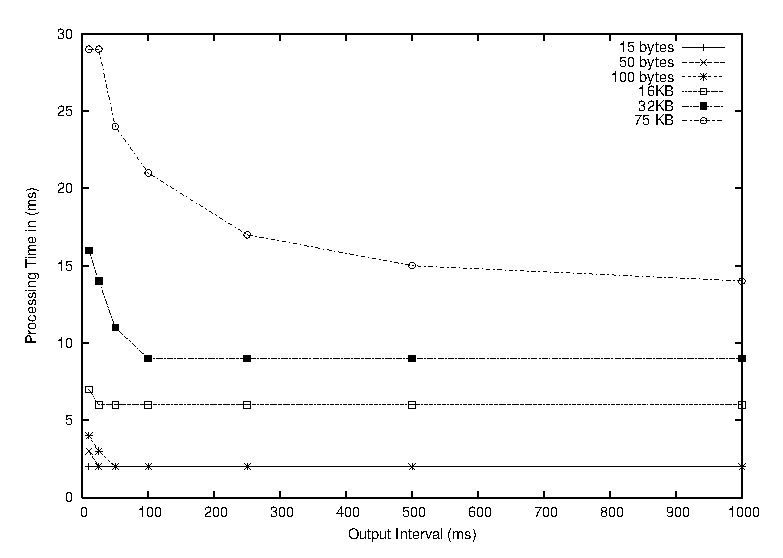
\includegraphics[width=0.8\columnwidth]{rates}
  \caption{GSN node under time-triggered load}
  \label{fig:TimeTriggeredLoad}
\end{figure}

High data rates put some stress on the system but the absolute delays are still
quite tolerable. The delays drop sharply if the interval is increased and then
converge to a nearly constant time at a rate of approximately 4 readings/second
or less. This result shows that GSN can tolerate high rates and incurs low
overhead for realistic rates as in practical sensor deployments lower rates are
more probable due to energy constraints of the sensor devices while still being
able to deal also with high rates.


\subsection{Scalability in the number of queries and clients}
\label{sec:scal-towards-numb}

In this experiment the goal was to measure GSN's scalability in the number of
clients and queries. To do so, we used two 1.8 GHz Centrino laptops with 1GB
memory as shown in Figure~\ref{fig:ExperimentalSetup} which each ran 250
lightweight GSN instances. The lightweight GSN instance only included those
components that we needed for the experiment. Each GSN-light instance used a
random query generator to generate queries with varying table names, varying
filtering condition complexity, and varying configuration parameters such as
history size, sampling rate, etc. For the experiments we configured the query
generator to produce random queries with 3 filtering predicates in the
\texttt{where} clause on average, using random history sizes from 1 second up
to 30 minutes and uniformly distributed random sampling rates (seconds) in the
interval $[0.01,1]$.

Then we configured the motes such that they produce a measurement each second
but would deliver it with a probability $P<1$, i.e., a reading would be dropped
with probability $1-P>0$.  Additionally, each mote could produce a burst of $R$
readings at the highest possible speed depending on the hardware with
probability $B>0$, where $R$ is a uniformly random integer from the interval
$[1,100]$. I.e., a burst would occur with a probability of $P * B$ and would
produce randomly 1 up to 100 data items.  In the experiments we used $P=0.85$
and $B=0.3$. On the desktops we used MySQL as the database with the recommended
configuration for large memory systems.
Figure~\ref{fig:QueryProcessingLatency} shows the results for a stream element
size (SES) of 30 Bytes. Using SES=32KB gives the same latencies. Due
to space limitations we do not include this figure.

\begin{figure}%[htb]
  \centering
  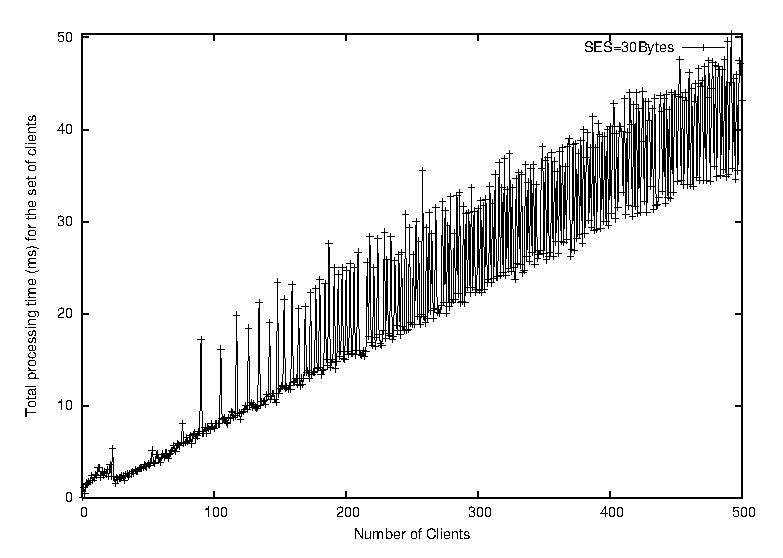
\includegraphics[width=0.8\columnwidth]{query-processing-time-30bytes}
%  \hspace{0.05\columnwidth}
%  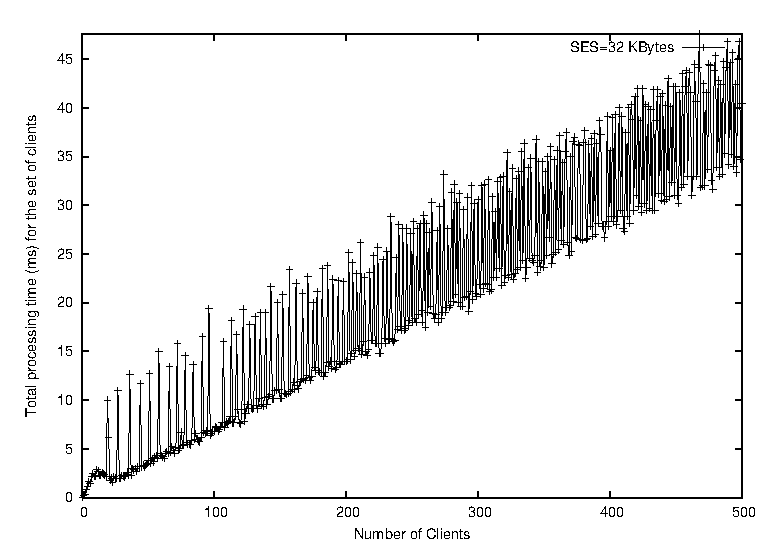
\includegraphics[width=0.45\columnwidth]{query-processing-time-32KB}
  \caption{Query processing latencies in a node}
  \label{fig:QueryProcessingLatency}
\end{figure}

The spikes in the graphs are bursts as described above. Basically this
experiment measures the performance of the database server under various loads
which heavily depends on the used database. As expected the database server's
performance is directly related to the number of the clients as with the
increasing number of clients more queries are sent to the database and also the
cost of the query compiling increases. Nevertheless, the query processing time
is reasonably low as the graphs show that the average time to process a query
if 500 clients issue queries is less than 50ms, i.e., approximately 0.5ms per
client. If required, a cluster could be used to the improve query processing
times which is supported by most of the existing databases already.

In the next experiment shown in Figure~\ref{fig:ProcessingTimePerClient} we
look at the average processing time for a client excluding the query processing
part. In this experiment we used $P=0.85$, $B=0.05$, and $R$ is as above. 

We can make three interesting observations from
Figure~\ref{fig:ProcessingTimePerClient}:

\begin{enumerate}
\item  GSN only allocates resources for virtual sensors that are being
  used. The left side of the graph shows the situation when the first
  clients arrive and use virtual sensors. The system has to instantiate
  the virtual sensor and activates the necessary resources for query
  processing, notification, connection caching, etc. Thus for the
  first clients to arrive average processing times are a bit
  higher. CPU usage is around 34\% in this interval. After a short
  time (around 30 clients) the initialization phase is over and the
  average processing time decreases as the newly arriving clients can
  already use the services in place. CPU usage then drops to around
  12\%.
  
\item Again the spikes in the graph relate to bursts. Although the processing
  time increases considerably during the bursts, the system immediately
  restores its normal behavior with low processing times when the bursts are
  over, i.e., it is very responsive and quickly adopts to varying loads.

\item As the number of clients increases, the average processing time
  for each client decreases. This is due to the implemented data
  sharing functionalities. As the number of clients increases, also
  the probability of using common resources and data items grows.
\end{enumerate}

\begin{figure}%[htb]
  \centering
  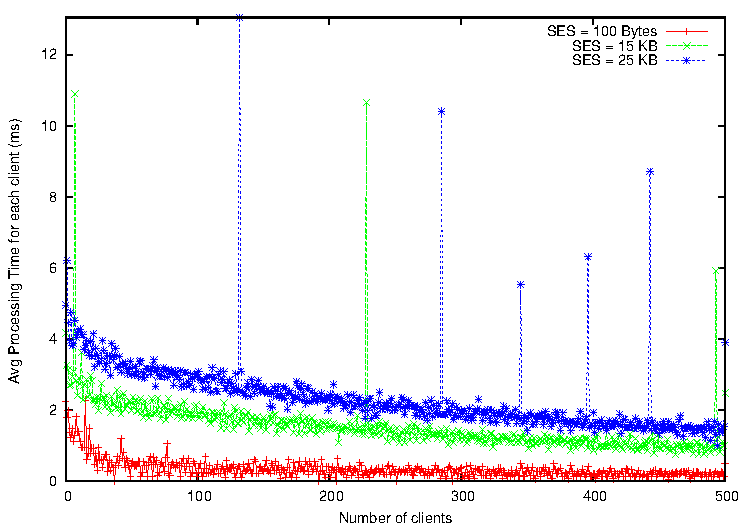
\includegraphics[width=0.8\columnwidth]{processing-time-per-client}
  \caption{Processing time per client}
  \label{fig:ProcessingTimePerClient}
\end{figure}

\section{Related work}
\label{sec:relatedwork}

So far only few architectures to support interconnected sensor networks exist.
Sgroi et al.~\cite{Sgroi05} suggest basic abstractions, a standard set of
services, and an API to free application developers from the details of the
underlying sensor networks.  However, the focus is on systematic definition and
classification of abstractions and services, while GSN takes a more general
view and provides not only APIs but a complete query processing and management
infrastructure with a declarative language interface.

Hourglass~\cite{Shneidman04} provides an Internet-based infrastructure for
connecting sensor networks to applications and offers topic-based discovery and
data-processing services. Similar to GSN it tries to hide internals of sensors
from the user but focuses on maintaining quality of service of data streams in
the presence of disconnections while GSN is more targeted at flexible
configurations, general abstractions, and distributed query support.

HiFi~\cite{Franklin05} provides efficient, hierarchical data stream query
processing to acquire, filter, and aggregate data from multiple devices in a
static environment while GSN takes a peer-to-peer perspective assuming a
dynamic environment and allowing any node to be a data source, data sink, or
data aggregator.

IrisNet~\cite{Gibbons03} proposes a two-tier architecture consisting of sensing
agents (SA) which collect and pre-process sensor data and organizing agents
(OA) which store sensor data in a hierarchical, distributed XML database. This
database is modeled after the design of the Internet DNS and supports XPath
queries. In contrast to that, GSN follows a symmetric peer-to-peer approach as
already mentioned and supports relational queries using SQL.

Rooney et al.~\cite{Rooney06} propose so-called EdgeServers to integrate sensor
networks into enterprise networks. EdgeServers filter and aggregate raw sensor
data (using application specific code) to reduce the amount of data forwarded
to application servers. The system uses publish/subscribe style communication
and also includes specialized protocols for the integration of sensor
networks. While GSN provides a general-purpose infrastructure for sensor
network deployment and distributed query processing, the EdgeServer system
targets enterprise networks with application-based customization to reduce
sensor data traffic in closed environments.

Besides these architectures, a large number of systems for query processing in
sensor networks exist. Aurora~\cite{Cherniack03} (Brandeis University, Braun
University, MIT), STREAM~\cite{Arasu06} (Stanford),
TelegraphCQ~\cite{Chandrasekaran03} (UC Berkeley), and Cougar~\cite{Yao03}
(Cornell) have already been discussed and related to GSN in
Section~\ref{sec:data-stre-proc}.

%The Aurora project~\cite{Cherniack03} is a general-purpose centralized stream
%processing engine. Streams are modeled as sequences of time-stamped tuples, and
%users can compose stream relationships and construct queries in a graphical
%representation which is then used as input for the query planner.

In the Medusa distributed stream-processing system~\cite{Zdonik03}, Aurora is
being used as the processing engine on each of the participating nodes. Medusa
takes Aurora queries and distributes them across multiple nodes and
particularly focuses on load management using economic principles and high
availability issues. The Borealis stream processing engine~\cite{Abadi05} is
based on the work in Medusa and Aurora and supports dynamic query modification,
dynamic revision of query results, and flexible optimization. These systems
focus on (distributed) query processing only, which is only one specific
component of GSN, and focus on sensor heavy and server heavy application
domains.

Additionally, several systems providing publish/subscribe-style query
processing comparable to GSN exist, for example, \cite{Gray05}.

\section{Conclusions}
\label{sec:conclusions}

The full potential of sensor technology will be unleashed through large-scale
(up to global scale) data-oriented integration of sensor networks. To realize
this vision of a ``Sensor Internet'' we suggest our Global Sensor Networks
(GSN) middleware which enables fast and flexible deployment and interconnection
of sensor networks. Through its virtual sensor abstraction which can abstract
from arbitrary stream data sources and its powerful declarative specification
and query tools, GSN provides simple and uniform access to the host of
heterogeneous technologies. GSN offers zero-programming deployment and
data-oriented integration of sensor networks and supports dynamic configuration
and adaptation at runtime. Zero-programming deployment in conjunction with
GSN's plug-and-play detection and deployment feature provides a basic
functionality to enable sensor mobility. GSN is implemented in Java and C/C++
and is available from SourceForge at \url{http://gsn.sourcefourge.net/}.
The experimental evaluation of GSN demonstrates that the implementation is
highly efficient, offers very good performance and throughput even under high
loads and scales gracefully in the number of nodes, queries, and query
complexity.




